%\subsection{$\boldsymbol{R_{e/\mu}}$ and lepton flavor universality}

The branching ratio 
%\begin{equation}
$R_{e/\mu} = \frac{\Gamma\left(\pi^+ \rightarrow e^+ \nu (\gamma) \right)}{\Gamma\left(\pi^+ \rightarrow \mu^+ \nu (\gamma)\right)}$
%\end{equation}
for pion decays to electrons over muons provides the best test of electron--muon universality in charged-current weak interactions. In the Standard Model (SM), $R_{e/\mu}$ has been calculated with extraordinary precision at the $10^{-4}$ level as \cite{Cirigliano1,Cirigliano2,Bryman1}
\begin{equation}
\label{Remu_SM}
    R_{e/\mu} \hspace{0.1cm}\text{(SM)} = (1.2352\pm 0.0002)\times10^{-4},
\end{equation}
perhaps the most precisely calculated weak interaction observable involving quarks. Because the
uncertainty of the SM calculation for $R_{e/\mu}$ is very small and the decay $\pi^+ \rightarrow e^+ \nu$ is helicity-suppressed by the $V-A$ structure of charged currents, a measurement of $R_{e/\mu}$ is extremely sensitive to the presence of pseudo-scalar (and scalar) couplings absent from the SM; a disagreement with the theoretical expectation would unambiguously imply the existence of new physics beyond the SM. With measurements of 0.01\% experimental precision, new physics beyond the SM (BSM) up to the mass scale of 3000 TeV may be revealed by a deviation from the precise SM expectation \cite{Bryman1}. Possible sources of deviation include new interactions involving scalar particles like Majorons \cite{Lessa}, charged Higgs particles, and leptoquarks \cite{Campbell}. Supersymmetry models with and without $R$-parity violation \cite{Ramsey-Musolf} or with lepton flavor violating terms \cite{Masiero} could also cause deviations from the SM prediction. Other new physics effects which could modify $R_{e/\mu}$ include massive sterile neutrinos \cite{Bryman2} and dark sector processes such as $\pi^+ \rightarrow e^+ \nu \hspace{1mm}\textrm{X}$ \cite{Altmannshofer}, which are also sought in the rare pion decay experiments \cite{Aguilar-Arevalo1, Aguilar-Arevalo2}. 

\paragraph{}
Currently, the most accurate measurement was reported by PIENU \cite{Aguilar-Arevalo3},
\begin{equation}
\label{Remu_exp}
     R_{e/\mu} \hspace{0.1cm} \text{(Expt)} = (1.2344 \pm 0.0023 (\text{stat}) \pm 0.0019 (\text{syst})) \times 10^{-4},
\end{equation}
 at the 0.2\%  precision level. It corresponds to a test of $e$--$\mu$ universality $g_e/g_\mu = 0.9996 \pm 0.0012$, expressed as the ratio of potentially distinct weak couplings for the electron and muon. The result is in excellent agreement with the SM expectation in contrast to recent hints of violation of third generation lepton flavor universality in some $B$-meson decays \cite{LFVB}. The goals of the present TRIUMF PIENU \cite{Aguilar-Arevalo4, Aguilar-Arevalo5} and PSI PEN \cite{Pocanic1, Pocanic2, Pocanic3} experiments are to improve the measurement precision by another factor of 2 or more to a level of $<0.1\%$. However, even if these goals are realized, this still leaves room for experimental improvement by more than an order of magnitude in uncertainty to confront
the SM prediction and to search for BSM effects. The goal of a future experiment discussed below would be a further improvement in precision by an order of magnitude to 0.01\%, making the
experimental uncertainty comparable to the theoretical uncertainty.

%\subsection{Pion beta decay}


\begin{figure}[t!]
\centering
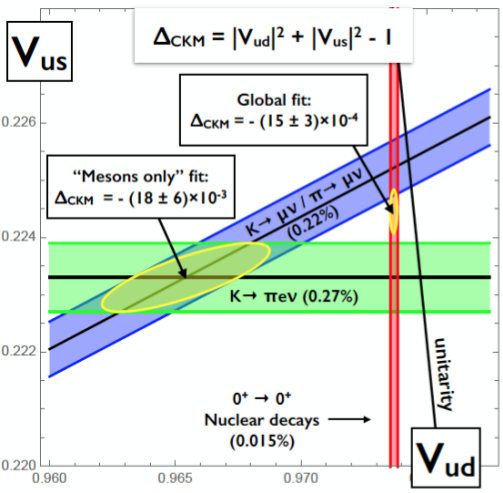
\includegraphics[scale=0.5]{sections/figures/fig-ckm.png}
\caption{Existing tensions in the 1st-row CKM unitarity test.}
\label{fig:CKM}
\end{figure}


The uncertainty of the SM prediction~\eqref{Remu_SM} for $R_{e/\mu}$ arises from low-energy constants in chiral perturbation theory, which absorb the divergences in the two-loop calculation of Refs.~\cite{Cirigliano1,Cirigliano2}, but whose finite parts need to be determined by other means. Fortunately, in the case of  $R_{e/\mu}$ these nonperturbative uncertainties only affect the SM prediction at the relative precision of $10^{-4}$, more than an order of magnitude beyond the current experimental precision~\eqref{Remu_exp}. $R_{e/\mu}$ thus provides a unique opportunity for a pristine test of lepton flavor universality (LFU) in the quark sector. 

While no particles beyond the ones of the SM have been observed so far at the LHC, experiments have accumulated intriguing hints for the violation of LFU (LFUV) within recent years. In particular, the measurements of the ratios $R(D^{(*)})$~\cite{Lees:2012xj,Aaij:2017deq,Abdesselam:2019dgh} and $R(K^{(*)})$~\cite{Aaij:2017vbb,Aaij:2019wad} deviate from the SM expectation of LFU by more than $3\sigma$~\cite{Amhis:2019ckw,Murgui:2019czp,Shi:2019gxi,Blanke:2019qrx,Kumbhakar:2019avh} and $4\sigma$~\cite{Alguero:2019ptt,Aebischer:2019mlg,Ciuchini:2019usw,Arbey:2019duh}, respectively. In addition, the anomalous magnetic moments $(g-2)_\ell$ of charged leptons also measure the violation of LFU as they vanish in the massless limit. Here, there is the long-standing discrepancy in $(g-2)_\mu$ of about $3.7\sigma$~\cite{Bennett:2006fi,Aoyama:2020ynm}. In addition, there is a $2\sigma$ tension in $\tau\to\mu\nu\nu/\tau\to e\nu\nu$~\cite{Aoki:2019cca}, and also the deficit in first-row CKM unitarity shown in Fig.~\ref{fig:CKM}  can be viewed as a sign of LFUV~\cite{Crivellin:2020lzu}. 

\begin{figure}[t!]
\centering
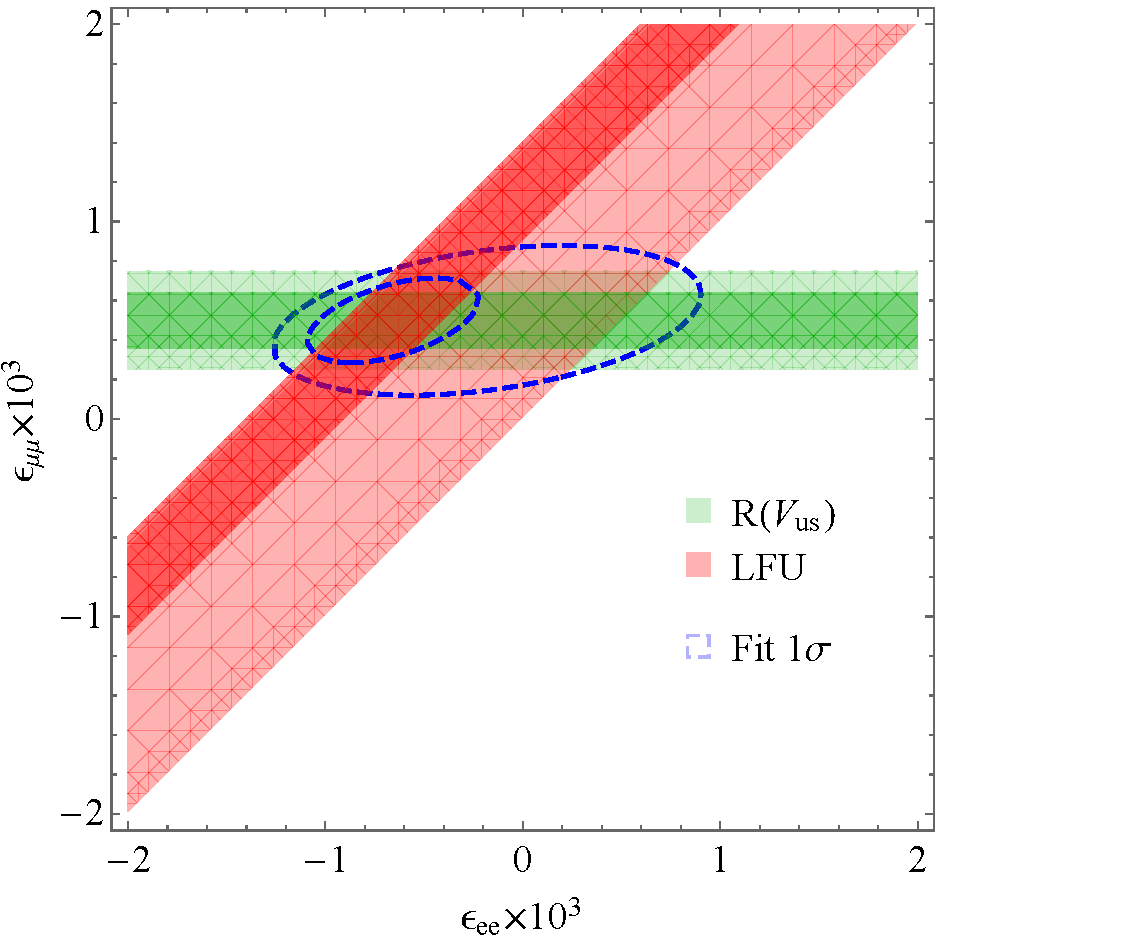
\includegraphics[scale=0.5]{sections/figures/Fit.pdf}
\caption{Modifications of the $W\ell\nu$ couplings, parameterized according to $\delta_{ij}+\epsilon_{ij}$~\cite{Crivellin:2020lzu}. The green bands refer to the constraint from $V_{ud}$ and $V_{us}$ via nuclear $\beta$ decays and kaon decays, the red band to other tests of LFU, dominated by $R_{e/\mu}$ and $\tau\to\mu\nu\nu/\tau\to e\nu\nu$. The light bands refer to the present situation, the dark ones to future projections.}
\label{fig:Fit_epsii}
\end{figure}

For the latter,  assuming that LFUV  originates from modified $W\ell\nu$ couplings, mainly the determination from $\beta$ decays is affected, due to a CKM enhancement by $(V_{ud} / V_{us})^2 \sim 20$. If this effect is real, and corrected for, the red band in Fig.~\ref{fig:CKM} will move to the left. Such a modification of the $W\ell\nu$ couplings would also affect $R_{e/\mu}$, albeit for a different flavor combination, see Fig.~\ref{fig:Fit_epsii}. 
In fact, this connection provides further motivation for the current proposal, especially because the sensitivity to LFUV would be comparable to future improved constraints from $\beta$ decays. Moreover, recent global fits to electroweak observables and tests of LFU show a preference for $R_{e/\mu}$ bigger than its SM expectation \cite{Coutinho:2019aiy,Crivellin:2020ebi}.









%\subsection{Pion beta decay}

The detector optimized for a next-gen $R_{e/\mu}$ experiment will also be ideally suited for a high-precision measurement of pion beta decay and searches for exotic pion and muon decays. Precision measurements of beta decays of neutrons,
nuclei, and mesons provide very accurate determinations of the elements $|V_{ud}|$ and $|V_{us}|$ of the
Cabibbo-Kobayashi-Maskawa (CKM) quark-mixing matrix \cite{Cabibbo, Kobayashi}. Recent theoretical
developments on radiative corrections and form factors have led to a $3\sigma$ tension with CKM
unitarity illustrated in Fig.~\ref{fig:CKM}, which, if confirmed, would point to new physics in the multi-TeV scale (see, e.g., Ref.~\cite{Czarnecki}).  
Pion beta decay, $\pi^+ \rightarrow \pi^0 e^+ \nu (\gamma)$, provides the theoretically cleanest determination of the CKM matrix element $V_{ud}$. With current input one obtains $V_{ud} = 0.9739(28)_{\textrm{exp}}(1)_{\textrm{th}}$, where the experimental uncertainty comes almost entirely from the  $\pi^+ \rightarrow \pi^0 e^+ \nu (\gamma)$ branching ratio (BRPB) \cite{Pocanic4} (pion lifetime contributes ${\delta}V_{ud} = 0.0001$), and the theory uncertainty has been reduced from $({\delta}V_{ud})_{\textrm{th}} = 0.0005$ \cite{Sirlin, Cirigliano3, Passera} to $({\delta}V_{ud})_{\textrm{th}} = 0.0001$ via a lattice QCD calculation of the radiative corrections \cite{Feng}. The current precision of 0.3\% on $V_{ud}$ makes $\pi^+ \rightarrow \pi^0 e^+ \nu (\gamma)$ not presently relevant for the CKM unitarity tests because super-allowed nuclear beta decays provide a nominal precision of %0.015\%. 
0.03\%. 



In order to make $\pi^+ \rightarrow \pi^0 e^+ \nu (\gamma)$ important for CKM unitarity tests, two precision experimental stages can be identified:
%\begin{enumerate}  
(1) As advocated in Ref.~\cite{Czarnecki}, a three-fold improvement in BRPB precision compared to Ref.~\cite{Pocanic3} would allow for a 0.2\% determination of $V_{us}/V_{ud}$ improving on measurement of  the ratio currently 
 %   \begin{equation}
      $  R_V = \frac{\Gamma\left(\textrm{K} \rightarrow \pi l \nu (\gamma) \right)}{\Gamma\left(\pi^+ \rightarrow \pi^0 e^+ \nu (\gamma)\right)}=1.3367(25)$ ,
 %   \end{equation}
    independent of the Fermi constant, short-distance, and structure-dependent radiative corrections. This
    would match the precision of the current extraction of $V_{us} / V_{ud}$ from the axial channels~\cite{Marciano} by making improvements to the current 
  % \begin{equation}
        $R_A = \frac{\Gamma\left(\textrm{K} \rightarrow \mu \nu (\gamma) \right)}{\Gamma\left(\pi \rightarrow \mu \nu (\gamma)\right)}=1.9884(115)(42)$,
 %   \end{equation}
    (see Fig. \ref{fig:CKM}), thus providing a new competitive constraint on the $V_{us}$--$V_{ud}$ plane and probing new physics that might affect vector and axial-vector channels in different ways.
    The theoretical case for this approach was recently strengthened by improved analysis of radiative corrections in $K \to \pi e \nu $ decays \cite{Seng:2021}.  
(2)  In the second phase, an order of magnitude improvement  in the
BRPB precision will be sought. This would provide the theoretically cleanest extraction of $V_{ud}$ at the 0.02\% level. 
%\end{enumerate}

High precision pion decay experiments can access rare and exotic decays, as  demonstrated by
previous experiments like PIENU. Extensions of the Standard Model postulate the
existence of additional (sterile) neutrinos \cite{nuMSM}\cite{BrymanShrock}. These additional states can potentially explain
the small mass of the SM neutrinos and contribute to the solution of outstanding puzzles like
the nature of dark matter  and early cosmological processes like small scale structure formation \cite{bertoni}.  
Exotic pion and muon decays involving sterile neutrinos  and axions in reactions including $\mu\to e a$\cite{Aguilar-Arevalo6},  $\pi \to l \nu_h$\cite{Aguilar-Arevalo1}\cite{Aguilar-Arevalo2} and $\pi \to l \nu a$\cite{Aguilar-Arevalo8} can provide new information on topical non-SM effects; the experiment proposed here will make improvements in sensitivity to such effects by an order of magnitude or more.


%\subsection{Searches for other rare and exotic decays}\label{Exotics}
High precision pion decay experiments can access rare and exotic decays, as  demonstrated by
previous experiments (see Fig~\ref{fig:decays}) like PIENU. Extensions of the Standard Model postulate the
existence of additional (sterile) neutrinos \cite{nuMSM}\cite{BrymanShrock}. These additional states can potentially explain
the small mass of the Standard Model neutrinos and contribute to the solution of outstanding puzzles like
the nature of dark matter  and early cosmological processes like small scale structure formation \cite{bertoni}.  
Massive neutrino states $\nu_H$ can be sought in the two-body pion decays
$\pi^+\rightarrow e^+\nu_H$ \cite{Aguilar-Arevalo1} and $\pi^+\rightarrow \mu^+\nu_H$ \cite{Aguilar-Arevalo2}. Exploiting
large datasets of pion decays and the resulting decay muons,  exotic two-body muon decays like $\mu^+\rightarrow e^+X$ can
be sought \cite{Aguilar-Arevalo6}, where X is a massive neutral boson (e.g. an axion or a Majoron).
Similarly, exotic particles have been searched for in three body decays like $\pi^+\rightarrow l^+ \nu X$ ($l=e^+,\mu^+$) \cite{Aguilar-Arevalo8}.
The PIENU experiment also obtained upper limits for the rare decays $\pi^+\rightarrow e^+\nu_e\nu\bar{\nu}$ and
$\pi^+\rightarrow \mu^+\nu_{\mu}\nu\bar{\nu}$ at the $10^6-10^7$ level \cite{Aguilar-Arevalo7}.\\
An experiment with two orders of magnitude more statistics has the potential to improve the existing limits by at least an order of magnitude.
Since the searches are based on a fit to the energy spectra of the visible final state particles, an improved experiment
can bring significant additional advantages in lowering the limits and in reducing the systematic errors. For example, 
the $\pi^+\rightarrow e^+\nu$ low energy tail represents a relevant background for the
$\pi\rightarrow e^+\nu_H$, $\pi^+\rightarrow e^+\nu X$, and $\pi^+\rightarrow e^+\nu_e\nu\bar{\nu}$ searches: 
more precise knowledge of the tail and its further reduction will significantly improve the upper limits beyond the statistics.
The search for rare and exotic decays involving  muons, like $\pi^+\rightarrow \mu^+\nu_H$, $\pi^+\rightarrow \mu^+\nu X$, and $\pi^+\rightarrow \mu^+\nu_{\mu}\nu\bar{\nu}$ will
benefit from an improved stopping target and faster electronics, which will allow better separation of  muons from pions and thus further improve the sensitivity.
Taking into account all the characteristics of an improved pion decay experiment, improvements by more than an order of magnitude can be expected.
\begin{figure}
    \centering
    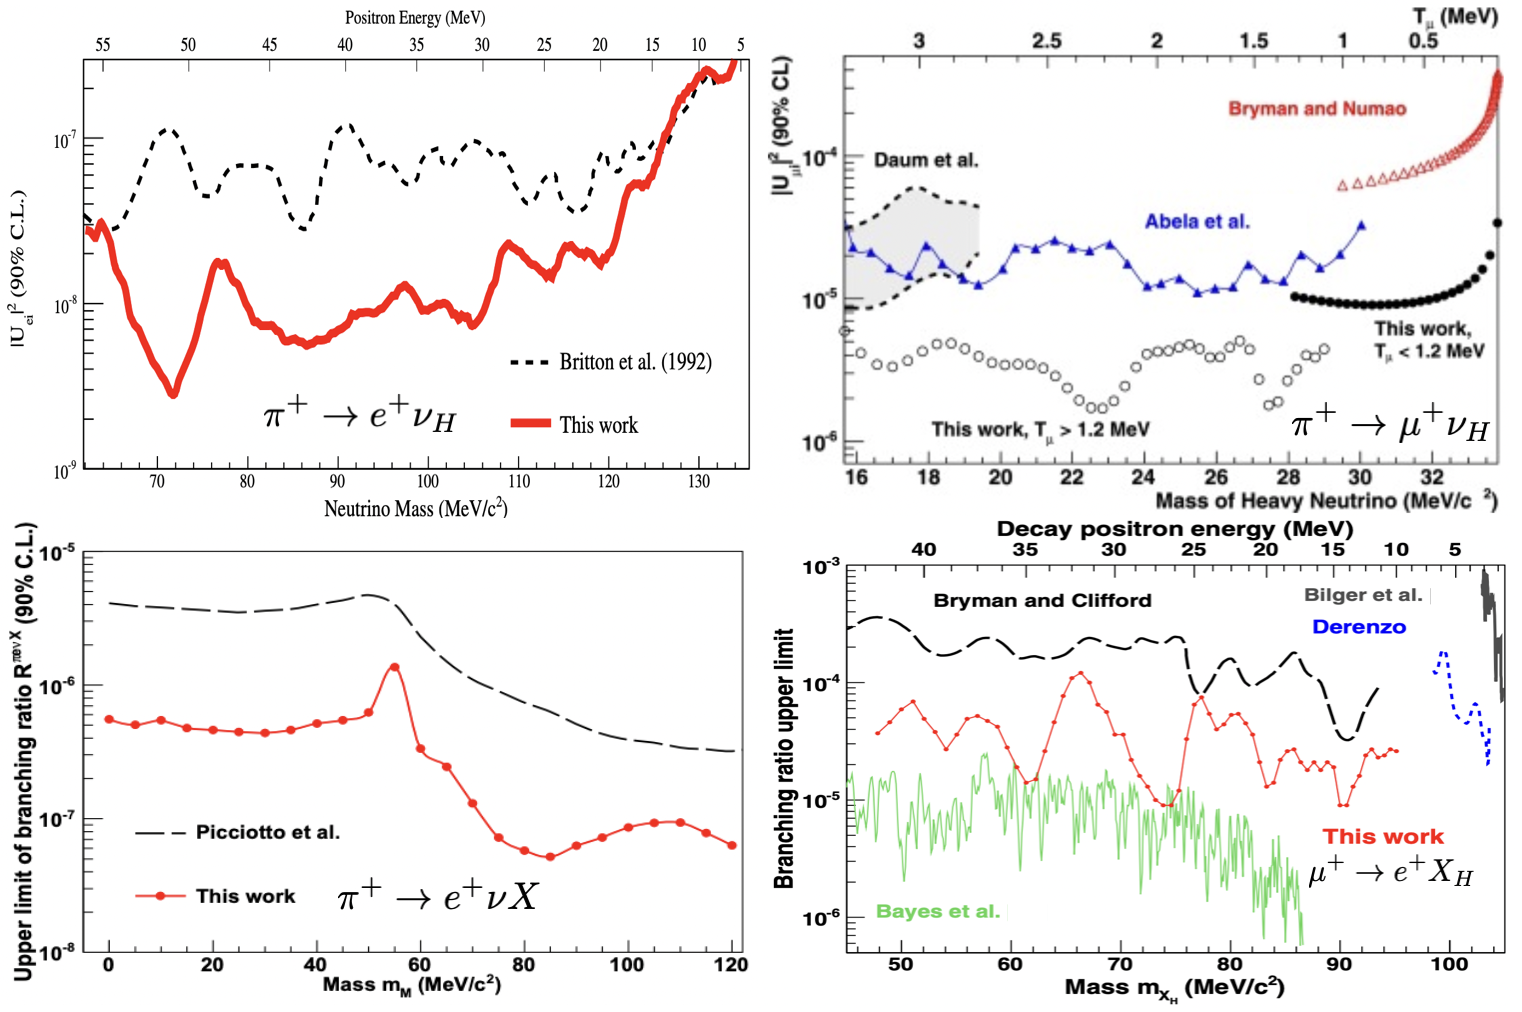
\includegraphics[width=0.6\textwidth]{sections/figures/RareResults.png}
    \caption{Exotic decay searches from the PIENU experiment. The 
    results are indicated with "This work" and show order of magnitude improvements in sensitivity over
    previous experiments.}
    \label{fig:decays}
\end{figure}


